\section{Desenvolvimento Experimental}
\subsection{Materiais e Métodos}
Foram utilizados para a realização do experimento:
\begin{itemize}
	\item Mini-laser;
	\item Mesa de alinhamento;
	\item Uma lente de 48 mm;
	\item Uma lente de 252 mm;
	\item Um separador de feixes;
	\item Um espelho de alta rotação PASCO OS-9263B;
	\item Um espelho fixo esférico com raio de 13,5 m;
\end{itemize}
Sendo o experimento montado da seguinte forma:
\begin{figure}[h!]
	\centering
	\fbox{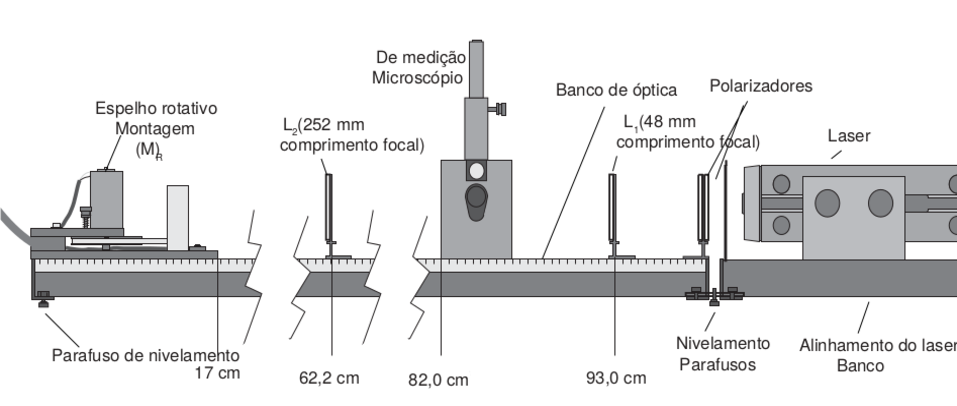
\includegraphics[scale= 0.35]{mtg}}
	\caption{Montagem experimental utilizada}
\end{figure}


Primeiro o laser e o espelho rotatório são alinhados sobre a mesa com o auxílio dos gabaritos, é posto então a primeira lente (48 mm), em seguida o separador de feixes e então a segunda lente (252 mm), é fundamental que ao colocar cada objeto óptico seja revisado seu alinhamento com o plano do laser. Utilizando regras trigonométricas, é posto então o espelho fixo esférico a cerca de 9 metros
do espelho giratório, formando entre eles um ângulo de aproximadamente 12º e, em seguida, alinhado seus centros observando  se o raio de luz está retornando ao separador de feixes. Nessa última etapa, é substituido a ocular do separador por um papel de pequena gramatura e, bloqueando o feixe de luz refletido pelo espelho rotatório, pode-se ver um ponto piscando no papel, o que significa que os espelhos estão alinhados. Por fim, é recolocado a ocular e alinhado o mostrador do micrômetro com o ponto de luz.
\subsection{Dados Obtidos Experimentalmente}
Após a realização do experimento, foram obtidos os dados que estão na
Tabela 1.
\begin{table}[h!]
\caption{Dados obtidos experimentalmente com seus respectivos erros}
\centering

\begin{tabular}{|	c	|	c	|}
\hline
$\Delta$ s'$\pm 2,5(mm)$ & $f \pm 1(Hz)$   \\ \hline
14          & 750   \\ \hline
30          & 1500  \\ \hline
-15         & -750  \\ \hline
-30         & -1500 \\ \hline
\end{tabular}
\end{table}

Utilizando os dados obtidos, foi gerado em programa o gráfico da
Figura 2,contendo o deslocamento do ponto ($\Delta$s') com a respectiva frequência ($f$) do espelho, e calculando o
ajuste linear obteve-se a equação da reta $\Delta s
=2.00\times10^{-7}f$.


\begin{figure}[!ht]
	\centering
		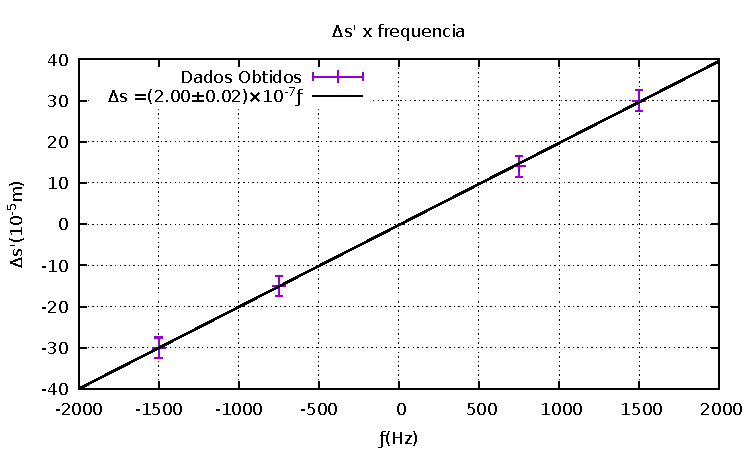
\includegraphics[scale= 1.1]{Graficusao/c.pdf}
	\caption{Relação entre deslocamento ($\Delta$s') do ponto e a
frequência ($f$) do espelho, com equação igual a $\Delta s
=(2.00\pm0.02)\times10^{-7}f$}
\end{figure}

\subsection{Interpretação dos Resultados}

Sabendo-se que
\begin{equation}
	c = \frac{4AD^22\pi f}{(D+B)\Delta s}
\end{equation}
é possível fazer
\begin{equation}
\begin{split}
	\Delta s = \frac{4AD^22\pi f}{(D+B)c}\\
	\Delta s = 2\times10^{-7}f
\end{split}
\end{equation}
portanto,
\begin{equation}
	2\times10^{-7}=\frac{8AD^2\pi}{(D+B)c}\\
\end{equation}
\begin{equation}
	c=\frac{8AD^2\pi}{(D+B)2\times10^{-7}}
\label{EQ}
\end{equation}
Substituindo os valores obtidos
\begin{equation}
	\begin{split}
		A = (0,261\pm0,0005)m\\
		B = (0,586\pm0,0005)m\\
		D = (9,485\pm0,0005)m
	\end{split}
\end{equation}
na equação \ref{EQ} obtem-se
\begin{equation}
	c=\frac{8*(0,261)*(9,485)^2*\pi}{[9,485+0,586]*2\times10^{-7}}
\end{equation}
e portanto
\begin{equation}
	c=(2,929\pm0,032)\times10^{8} m/s
\end{equation}
onde o valor de $0,032$ é obtido utilizando a equação \ref{eq:err}.\\
Comparado ao valor de 
\begin{equation}
	c=2,998\times10^{8} m/s
\end{equation}        
obtido na literatura \cite{PASCO}, resulta em um erro relativo ($Er$) de:
\begin{equation}
	Er=|\frac{2,929\times10^{8}-2,998\times10^{8}}{2,998\times10^{8}}|*100\%= 2,3\%
\end{equation}

Estes erros estão associados a montagem do experimento, sendo
possível um desalinhamento dos espelhos e lentes, além do feixe não estar colidindo exatamente no
centro do espelho fixo, o que acarreta uma variação do valor de $c$ predito na literatura. Porém, mesmo com todos os fatores associados, o erro  de
2,3\% é aceitável dentro da precisão necessária para a realização
do experimento.

